\documentclass{article}
\usepackage{amsmath,amsthm,amssymb,amsfonts}
\usepackage{setspace,enumitem}
\usepackage{graphicx}
\usepackage{hyperref}
\usepackage{natbib}
\usepackage{afterpage}
\usepackage{xcolor}
\usepackage{etoolbox}
\usepackage{booktabs}
\usepackage{pdfpages}
\usepackage{multicol}
\usepackage{geometry}
\usepackage{bbm}
\usepackage{csvsimple}
\usepackage{accents}
\hypersetup{
	colorlinks,
	linkcolor={blue!90!black},
	citecolor={red!90!black},
	urlcolor={blue!90!black}
}

\newtheorem{theorem}{Theorem}
\newtheorem{assumption}{Assumption}
\newtheorem{definition}{Definition}
\newtheorem{lemma}{Lemma}
\setlength{\parindent}{0cm}
\geometry{margin = 1in}

\newcommand{\R}{\mathbb{R}}
\newcommand{\ubar}[1]{\underaccent{\bar}{#1}}
\newcommand{\F}{\mathcal{F}}
% \newcommand{\H}{\mathcal{H}}
\newcommand{\xbf}{\mathbf{x}}
\newcommand{\Xbf}{\mathbf{X}}
\newcommand{\Vbf}{\mathbf{V}}
\newcommand{\zbf}{\mathbf{z}}
\newcommand{\Tbf}{\mathbf{T}}
\newcommand{\mubf}{\boldsymbol{\mu}}
\newcommand{\alphabf}{\boldsymbol{\alpha}}
\newcommand{\betabf}{\boldsymbol{\beta}}
\newcommand{\sigmabf}{\boldsymbol{\sigma}}
\newcommand{\onebf}{\mathbbm{1}}
\newcommand{\Covbf}{\text{\textbf{Cov}}}
\newcommand{\Varbf}{\text{\textbf{Var}}}

\newtoggle{extended}
\settoggle{extended}{false}

\title{FIN 971: PS5}

\author{Alex von Hafften}

\begin{document}

\maketitle

This problem set is to replicate Gomes (AER, 2001) ``Financing Investment".

\bigskip

The equilibrium wage, entrant mass, aggregate output, aggregate labor, and aggregate profits for our baseline specification (i.e. with financial frictions) and without financial frictions.  All equilibrium quantities are higher without financial frictions especially the mass of entrants.  This difference makes a lot of sense because all firms start with zero capital.

\bigskip

\csvautotabular{table_1.csv}

\section*{Question 1}

Below is a table that corresponds to Table 2 of Gomes (2001).  It features the aggregate results from the model. My numbers are generally inline with Gomes (2001) except for the external financing costs, which are about 10 times smaller (can see on rows 2 and 3).  I'm not exactly sure why; it could be to do  with how I'm aggregating.  But the share of floatation cost to external financing costs is close to Gomes (2001).

\bigskip

\csvautotabular{table_2.csv}

\bigskip

Below is a table that corresponds to Table 3 of Gomes (2001). It features the cross-sectional results from the model.  The average size is very different (possibly units).  The mean investment rate is close, but I find a lower standard deviation.  My mean Tobin's Q is close to Gomes (a little higher; closer to the data reported in Gomes).  The average cash flow is close, but the standard deviation is again lower.  The fraction of firms with negative investment is about half of Gomes.

\bigskip

\csvautotabular{table_3.csv}

\section*{Question 2}

Below is a table that breaks down the firm distribution based on the sign of their dividends.  Most firms are constrained that is they are not financed through seasoned equity injections but they are not paying out dividends either.  Due to using a capital grid, I defined constrained as $d \in (-\varepsilon, \varepsilon)$ instead of $d = 0$.  Thus, constrained includes firms with very small dividends as well.

\bigskip

\csvautotabular{table_4.csv}

\section*{Question 3}

For this question, I plot the franchise value, policy functions, and distributions.  I highlight the lowest productivity level in green, the median productivity level in red, and the highest productivity level in blue.

Below is a figure of the franchise value for different productivity and capital levels.  Franchise value is increasing both in productivity and capital.  The franchise values are tighter for low levels of capital across productivity levels and spread out as capital increases.

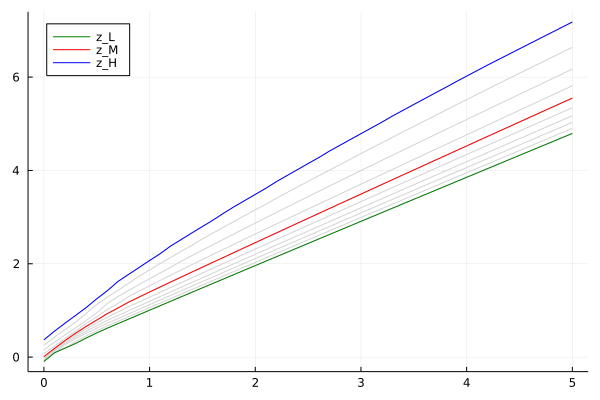
\includegraphics[scale = .5]{value_function.png}

\pagebreak

Below is a figure of the policy functions for capital, investment, continuation, and dividends.  Capital shows that highly productive firms are growing up to a certain size (i.e. the blue line is above the 45 degree line until $k \approx 4.25$) and as productivity drops the flattening out point drops.  This pattern is also mirrored in the investment policy function.  For certain productivity levels, investment is positive but it drops to negative at a certain point. From the dividend policy functions, we can see that these firms are growing through retained earnings instead of seasoned equity injections.  Only small and highly productive firms are funded through seasoned equity injection.  We can also see that only small low productivity firms exit the market.

\bigskip

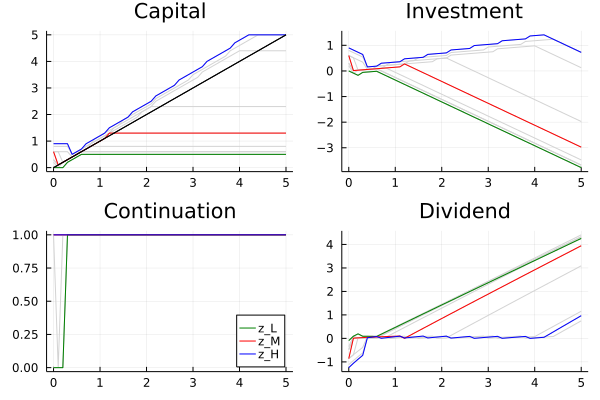
\includegraphics[scale = .75]{policy_functions.png}

\pagebreak

Below is a figure of the cumulative distribution functions based on productivity (i.e. all lines converge to one going to the right). This shows that all low productivity firms are small. And as productivity increases so does firm size.  The unconditional firm distribution across capital level is close to median productivity level because the distribution of firms across productivity levels is bell-shaped.

\bigskip

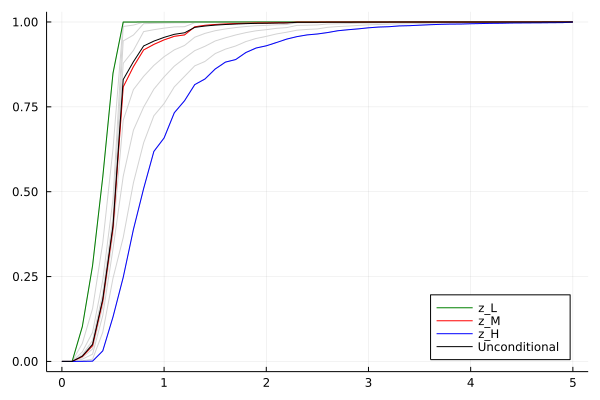
\includegraphics[scale = .5]{cdf.png}

\section*{Question 4}

I simulated a panel of 1200 firms for 10 years. First, I simulate the state transitions.  They all start from a random draw from $\phi(z_t)$.  Then to start the simulations of the capital, investment, continuation, and cash flows, I start the firms from a random draw from the stationary distribution for capital conditional on their initial productivity draw.  I initially tried starting all firms with zero capital, but since exit rates are higher for small firms, many of the firms immediately exited.  Then using the value and policy functions from the model computation, I simulate the paths of capital, investment, continuation, and cash flow.  In the table, I report the FHP regression based on these simulations in column (1). Standard errors are clustered at the firm-level. It makes sense that the coefficient on Tobin's Q is significant and positive.  The coefficient is significant and negative for cash-flow over lagged capital. It being significant is consistent with FHP, but it being negative is surprising.  This means that a higher cash-flow means lower investment.

\begin{table}[h]
\begin{tabular}{lrr}
\toprule
          & \multicolumn{2}{c}{investment} \\ 
\cmidrule(lr){2-3} 
          &       (1) &                (2) \\ 
\midrule
tobinq    &  0.797*** &              0.564 \\ 
          &   (0.058) &            (0.850) \\ 
cf        & -2.374*** &         -13.861*** \\ 
          &   (0.232) &            (2.114) \\ 
\midrule
year      &       Yes &                Yes \\ 
firm      &       Yes &                Yes \\ 
\midrule
Estimator &       OLS &                OLS \\ 
\midrule
$N$       &    10,320 &              3,837 \\ 
$R^2$     &     0.343 &              0.279 \\ 
\bottomrule
\end{tabular}

\end{table}

\pagebreak

\section*{Question 5}

I estimated the model without financial frictions (i.e. $\lambda_0 = \lambda_1 = 0$) in column (2) of the table above.  We see that the coefficient is still negative and significant suggesting that investment is still sensitive to cash flow even without financial frictions.  I was struck by how many more firms exit the market, so I plotted the value and policy functions and distributions without financial frictions (see below).  Firstly, it is striking that all concaving of the value and policy functions disappear, which makes sense because firms are risk-neutral.  Furthermore, all firms that are below the median productivity level exit the market.  This is consistent with the higher price and the higher mass of entrants from the first table.  The distributions confirm that are very few low productivity firms staying in the market.  In fact, the only firms are recent entrants that drew a low productivity and are planning on exiting.

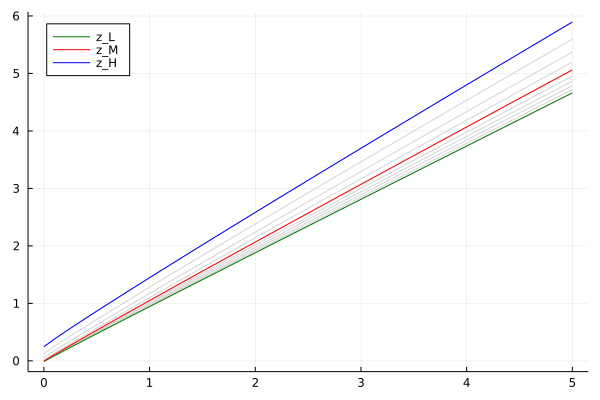
\includegraphics[scale = .5]{value_function_frictionless.png}

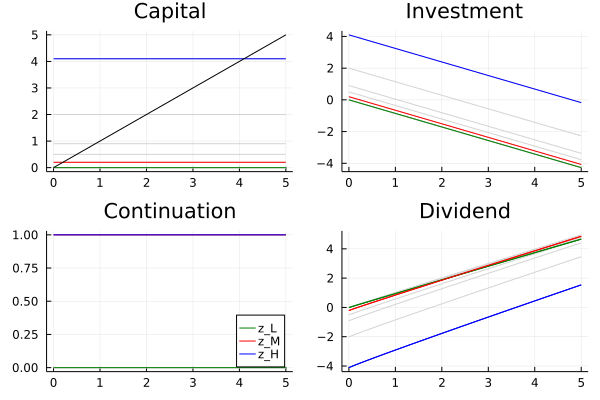
\includegraphics[scale = .5]{policy_functions_frictionless.png}

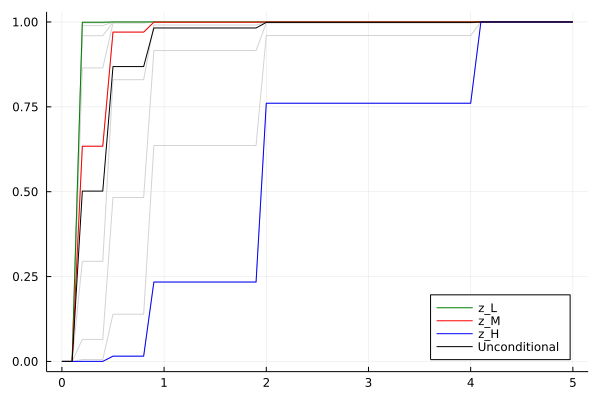
\includegraphics[scale = .5]{cdf_frictionless.png}


\end{document}

